\documentclass{article}
\usepackage[utf8]{inputenc}
\usepackage{xcolor}
\usepackage{graphicx}
\usepackage{amsmath}
\usepackage{amsthm}
\usepackage[english]{babel}

\newtheorem{theorem}{Theorem}[section]
\newtheorem{lemma}[theorem]{Lemma}

% Switch comments on / off
\def\marrow{{\marginpar[\hfill$\longrightarrow$]{$\longleftarrow$}}}
%\def\marrow{}
\def\mees#1{{\sc \textcolor{blue}{Mees says: }}{\marrow\sf \textcolor{red}{#1}}}
%\def\mees#1{}


\title{Physics-based trajectory outlier detection (working title)}
\author{Bram Custers, Mees van de Kerkhof, Wouter Meulemans,\\ Bettina Speckmann, Frank Staals}
\date{November 2018}

\begin{document}

\maketitle

\section{Introduction}
The use of GPS trajectories in computing has greatly increased in recent years. There are many algorithms and applications that use them as input. However, since the trajectories are a result of real-world measurements there is always some amount of error. Thus, no matter the application, it can be useful to preprocess trajectories to try and reduce the impact the error has on our result. 
There are several types of preprocessing that can be applied to a trajectory to limit the impact of errors, such as trajectory smoothing techniques, reducing the amount of measurements by trajectory smoothing, doing calculations assuming uncertain trajectory data etc.
This paper focuses on trajectory outlier detection. This problem as already been approached from a variety of angles. 

We approach the problem from a physics perspective. Trajectories track real-world objects with real-world physical properties. By considering if the tracked object could physically travel between its measured points in the given time interval we can find outlying points. 
We study several different problems using this idea of physical limitations. In general, we consider a subset of measurements of a trajectory to be \emph{consistent} if there is a path the object could have taken that covers the points and is consistent with the physics model. Our problem is then to find the maximum consistent subset of the trajectory.

\section{Definitions \& Notation}
A trajectory \(T=\{p_1,p_2,\dots,p_n\}\) is an ordered series of \(n\) \emph{measurements}. Which information is included in a measurement varies between problems, but it always includes some sort of specification of location as well as a timestamp. These timestamps are denoted \(t_i\), for each measurement \(p_i\). Since the measurements are sorted on time we have that \(t_i < t_{i+1},  \forall i\). We can divide a trajectory into \emph{subtrajectories}, which are denoted as follows: \(T[i,j]=\{p_k \in T | i \leq k \leq j\}\).
If the object being tracked can move from measurement \(p_i\) to measurement \(p_j\) (with \(j>i\)) without violating any physical constraints, we say \(p_i\) and \(p_j\) are \emph{consistent}. We call a larger subset of measurements consistent iff the object can visit each of the measurements in order without violating physical constraints. 
We denote the consistency of a set of measurements \(S\) as \(C(S)\). If the set is not consistent we write \(\neg C(S)\).
Depending on the physical model, we can be interested in the speed of the tracked object at the time of each measurement. We say that a pair of measurements \(p_i, p_j\) with \(j>i\) is \emph{speed-consistent} for a given speed \(s\) iff the object can travel from \(p_i\) to \(p_j\) and have a speed of \(s\) at \(t_j\) without violating physical constraints. We denote speed-consistency of a pair \(p_i, p_j\) for speed \(s\) as \(C_s(p_i,p_j)\). If the pair is not speed-consistent for this speed, we denote it as \(\neg C_s(p_i,p_j)\).

\section{Cubic algorithm for 1D trajectories}
\label{sec:1dspeedless}
Let \(T\) be a trajectory, where each measurement is of the form \(p_i=\{x_i,t_i\}\). So it has a 1-dimensional position, and a timestamp. We assume the object has a maximum speed \(s_{max}\) and a maximum acceleration \(a_{max}\) and deceleration \(d_{max}\). For the purpose of our model we assume there are no other physical constraints on the object.
Testing if two points \(p_j\) and \(p_{j+1}\) are consistent is easy, as we can check if the distance divided by the time difference falls under \(s_{max}\) and if there exists a starting speed for \(p_j\) such  required speeds can be reached by accelerating. However, when considering more than two points, the situation becomes more complicated. Whether or not \(p_{j+1}\) is reachable from \(p_j\) may depend on the speed the object has at \(t_j\), and likewise, there may only be a limited range of speeds the object can have at time \(t_{j+1}\) if it came from \(p_j\). So we can have the case where \(C(\{p_j,p_{j+1}\})\),\(C(\{p_j,p_{j+2}\})\),\(C(\{p_{j+1},p_{j+2}\})\), but \(\neg C(\{p_j,p_{j+1},p_{j+2}\})\)! See Figure~\ref{fig:speedproblem} for an example.

\begin{figure}
    \centering
    \fbox{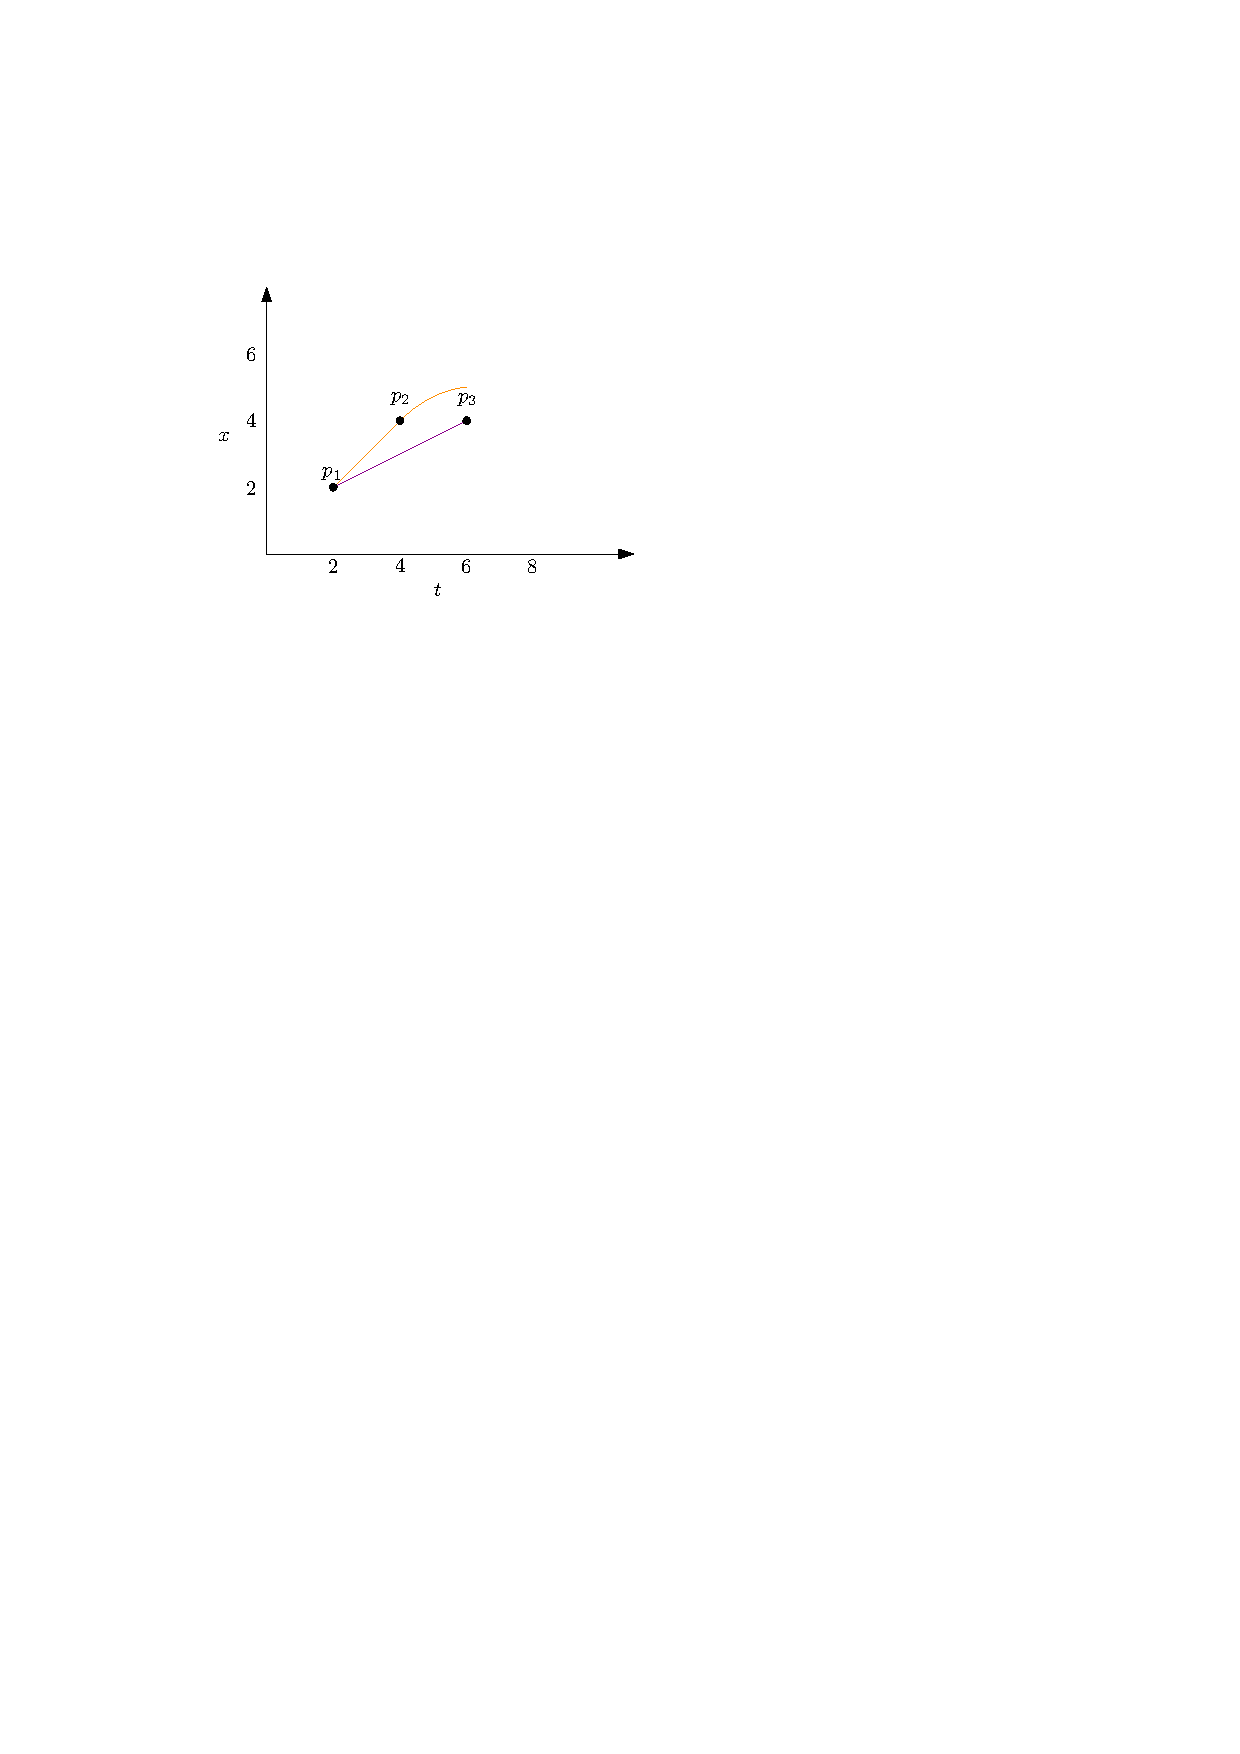
\includegraphics{figures/speedproblem.pdf}}
    \caption{Example trajectory, with \(s_{max}=1, d_{max}=0.5\). \(p_1\) and \(p_2\) are compatible, but only if the object is moving at maximum speed until \(t_2\) (the orange curve). \(p_1\) and \(p_3\) are also compatible, e.g. by following the purple curve, but there is no way to go from \(p_1\) to \(p_3\) while visiting \(p_2\), even if braking maximally after \(t_2\).}
    \label{fig:speedproblem}
\end{figure}

To solve this problem, we use dynamic programming. We maintain an array \(D: X \times X \mapsto I\), where \(X=\{1,\dots,n\}\) and \(I\) is a set of speeds between \(-s_{max}\) and \(s_{max}\). \(D(k,i)\) stores the possible speeds the object can have at \(t_i\) if it has to visit exactly \(k-1\) measurements from \(T[1,i-1]\) and end at \(p_i\). \(I\) always consists of a series of intervals. This is due to the following Lemma:
\begin{lemma}
If \(C_{s_1}(p_i,p_j) \land C_{s_2}(p_i,p_j)\) then \(C_s(p_i,p_j)\quad\forall s: s_1 \leq s \leq s_2\). 
\end{lemma}
\begin{proof}
To be added.
\end{proof}

For this algorithm to work in cubic time, it is important that the number of intervals in any \(D[k,i]\) is bounded. It is very easy to create a situation where a \(D[k,i]\) has more than one interval, see Figure~\ref{fig:twointervals}.

\begin{figure}
    \centering
    \fbox{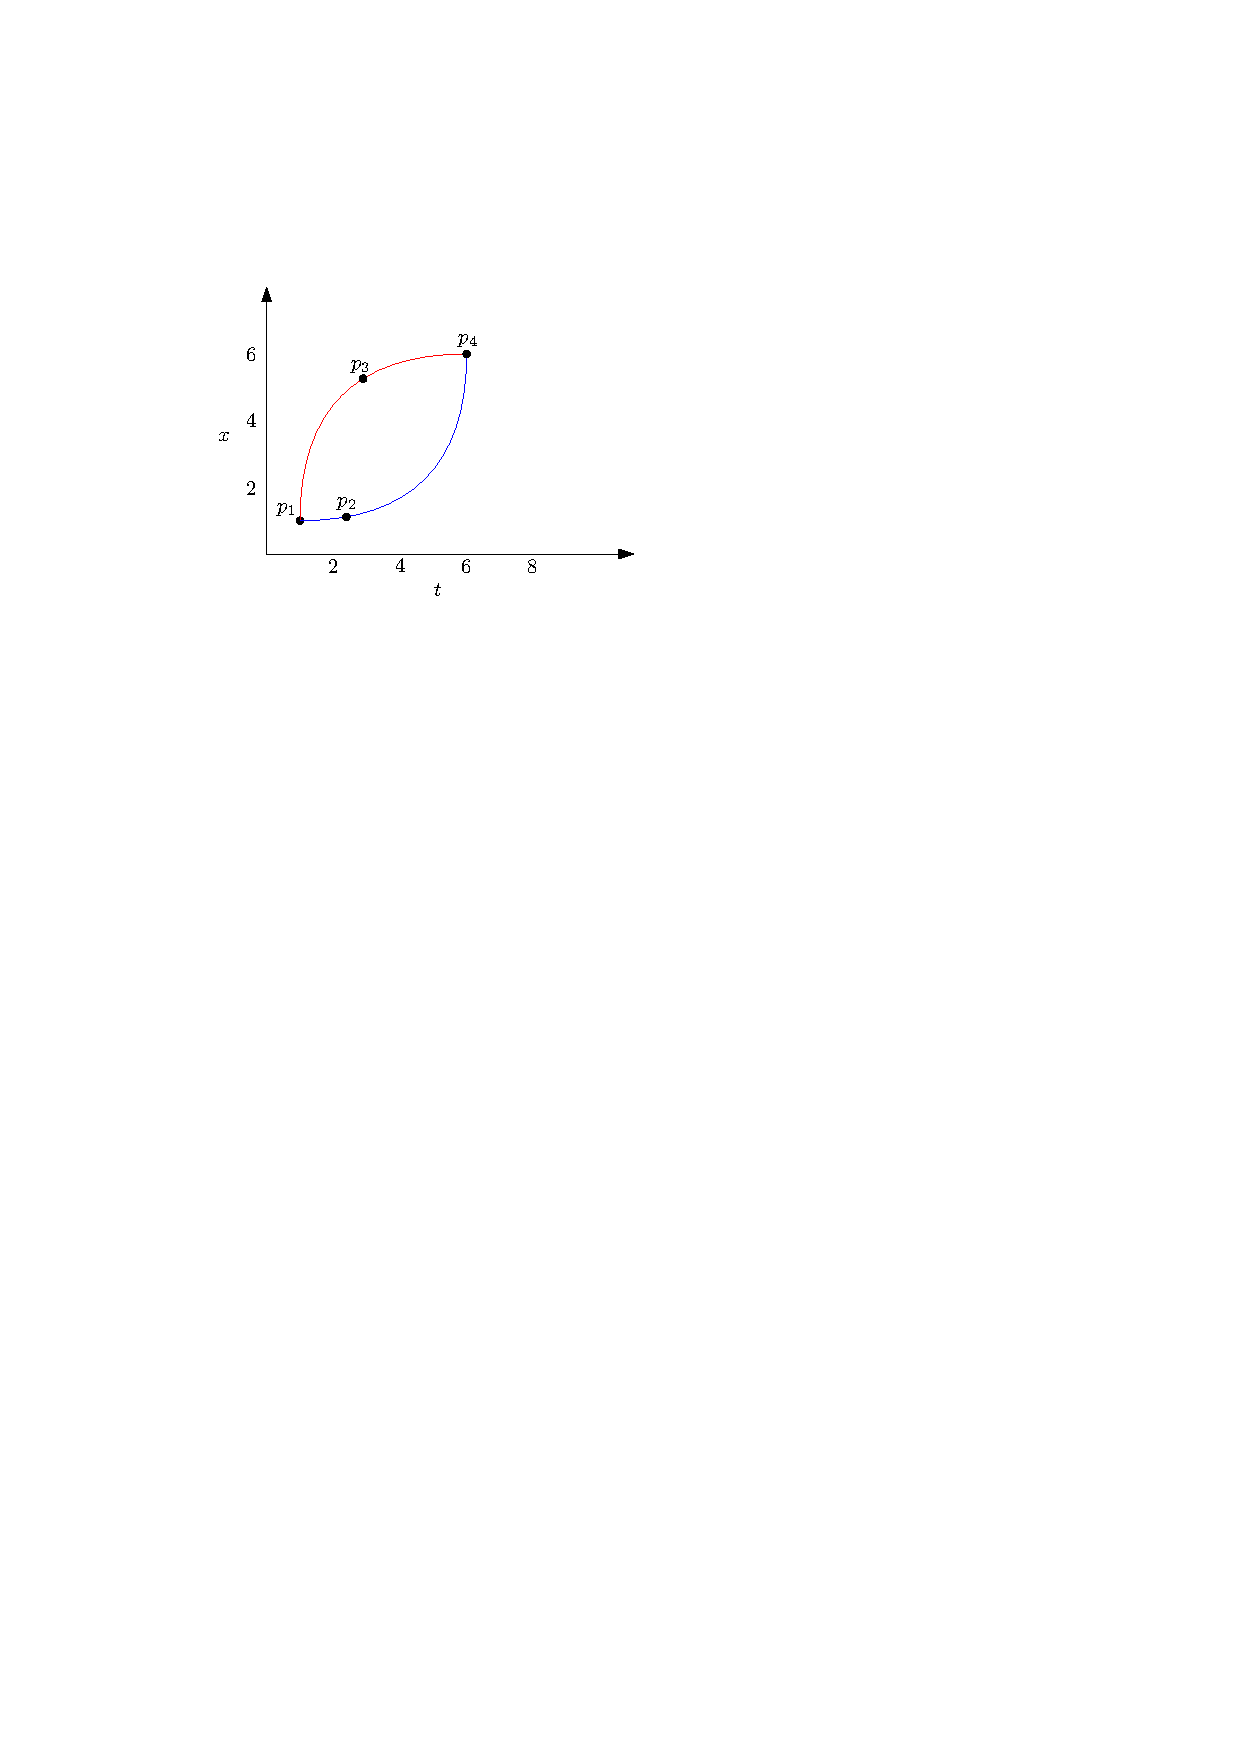
\includegraphics{figures/twointervals.pdf}}
    \caption{The red curve corresponds to maximal braking after \(p_1\), the blue curve to maximal acceleration. Because \(p_2\) and \(p_3\) are placed on these opposite curves, \(D[3,4]\) has two disjoint intervals: One where the object has maximum speed, the other where it has just slowed to a near standstill.}
    \label{fig:twointervals}
\end{figure}

The question of how many intervals any \(D[k,i]\) can maximally have is related to how the intervals propagate from one measurement to the next. To find the intervals for \(D(k,i)\), we can propagate the intervals forward from \(D(k-1,j)\) for \(k-1 \leq j < i\). We can do this as follows:\\ \(<\)INSERT TRICKY ACCELERATION MATH HERE\(>\)

\section{Subquadratic algorithm for 2D trajectories}
\label{sec:2Dcones}
Let \(T\) be a trajectory, where each measurement is of the form \(p_i=\{x_i,y_i,t_i\}\). So it has 2-dimensional coordinates for its position. We assume the tracked object has a maximum speed \(s_{max}\). For this model, we assume there are no other physical constraints on the object.
Because there is no longer a bound on acceleration, we do not have the problem of Section~\ref{sec:1dspeedless} where pairs of points that are consistent may not be consistent when put together. This allows us to solve the problem much faster.
We handle the measurements of our trajectory in order. For each measurement, we store the length of the longest consistent subset of \(T\) ending in that measurement. By storing this in an interval tree, we can query the tree with an integer \(k\) in \(O(\log n)\) time and get every measurement that has a consistent path going to it of at least length \(k\).  
Consider the measurements of the trajectory as existing in a 3D space, where time is the vertical axis. We can find all possible measurements that would be consistent with a measurement \(p_i\) by projecting a cone into space where \((x_i,y_i)\) are the coordinates of the tip and the radius of the cone at a time \(t_j > t_i\) is equal to \(s_{max}\cdot (t_j-t_i)\). Any measurement that lies within this cone is consistent with \(p_i\). 
Lets say we have processed the first \(i-1\) measurements of \(T\) and now want to handle measurement \(p_i\). If we query our interval tree for a given \(k\) we get a set of measurements \(P\) which were handled before \(p_i\) that permit a consistent path of length at least \(k\). If any of them are consistent with \(p_i\) we know that there is a path of length at least \(k+1\) ending in \(p_i\). Going back to the 3D representation we know that if one of the cones projected from  \(P\) contains \(p_i\) such a path must exist. If we project these cones onto the plane described by \(t=t_i\) we get a set of circles. We can build a power diagram out of these circles. By cleverly storing partial power diagrams we can do this in \(O(\log^2 n)\) time. \mees{I still need to look up exactly how this clever storage works, or someone else can add this part of the description. Its something with data structures of logarithmically growing sizes}. By querying this power diagram with the point \((x_i,y_i)\) we know which of the cones is closest to \(p_i\). We can then check if this cone contains \(p_i\). If it doesn't, we know none of the cones do and there does not exist a path of length \(k+1\) ending in \(p_i\). 
By performing a binary search on the largest \(k\) that gives a cone containing \(p_i\) we can find the longest path ending in \(p_i\) in \(O(\log^3 n)\) time. Doing this for all measurements means our algorithm runs in \(O(n\log^3 n)\)

\section{Output-sensitive algorithm}
Let \(T\) be a trajectory, where each measurement is of the form \(p_i=\{x_i,y_i,t_i,v_{x_i},v_{y_i}\}\). The measurements have 2-dimensional coordinates, a timestamp, and a velocity vector $\vec{v_i}= \begin{bmatrix} v_{x_i} \\ v_{y_i} \end{bmatrix}$. We assume the object has a maximum speed \(s_{max}\) and a maximum acceleration \(a_{max}\) and deceleration \(d_{max}\). For the purpose of our model we assume there are no other physical constraints on the object.
Once again we escape the problem of Section~\ref{sec:1dspeedless}. Since the velocity at the time of each measurement is given, there is no possibility that two measurements are only compatible for certain speeds that may be incompatible with other, otherwise consistent, measurements.
Since our physics model is more sophisticated again, we cannot use the algorithm given in Section~\ref{sec:2Dcones}. We no longer have nicely shaped cones in the 3D-representation, as the radius at any time depends on the speed the object has at all moments in between.
We can still solve this problem in quadratic time, however. To do this we construct a DAG. Let \(G=(V,A)\) be a graph with a vertex for each measurement of \(T\) and an arc from a vertex to another if the later vertex's measurement can be reached from the earlier one. This graph has \(O(n^2)\) complexity. We can then take the longest path in this graph in \(O(|V|+|A|)\) time. The measurements associated with the vertices in this longest path form the largest consistent subset of \(T\).
Although we do not further improve this quadratic time bound in an absolute way, we can modify the algorithm to an output-sensitive version that runs in \(O(nd)\) time, where \(d\) is the number of outliers:
Once again we handle the measurements one at a time. We maintain a linked list that stores all of the measurements that have already been handled, sorted in decreasing order of the largest length of a path that ends in that measurement. For handling a new measurement, we go down this list in order, stopping as soon as we find a measurement that is consistent with the new one. We then know that the length of the longest path ending in the new measurement is equal to the length of the path ending in this previous measurement plus 1. After we have handled all measurements in this way we know the longest path.
To see why this gives a \(O(nd)\) time bound we consider the fact that when we check the consistency between two measurements and get a negative result, at least one of the two measurements cannot be in the longest path and must be an outlier. This, combined with the fact that we stop checking a measurement against the rest as soon as we find a consistent pair means the following:

There are \((n-d)\) measurements which will end up in the maximal consistent subset. For each of these measurements, we will do one (1) check to find consistency with the previous measurement in the maximal consistent subset. Before we do that check, we have to make at most \(d\) checks as we fail to find consistency with what will later prove to be outliers.
Besides those measurements there are the \(d\) outliers, for each of these we will have to make at most \(n-1\) checks, as we pass over every previously handled measurement but fail to find any consistency.
Together this means we make \((n-d)(1+d) + d(n-1)\) checks, which works out to \(O(nd)\).

\section{Experiments}
\section{Conclusion}
\section{Acknowledgement}
This work was initiated at the 4th AGA workshop, using funds from the NWO.
\end{document}
